\documentclass[aspectratio=1610,onlymath]{beamer}
\setbeamertemplate{navigation symbols}{}
\usepackage{graphicx}
\begin{document}

\begin{frame}
\begin{figure}[ht]
\centering
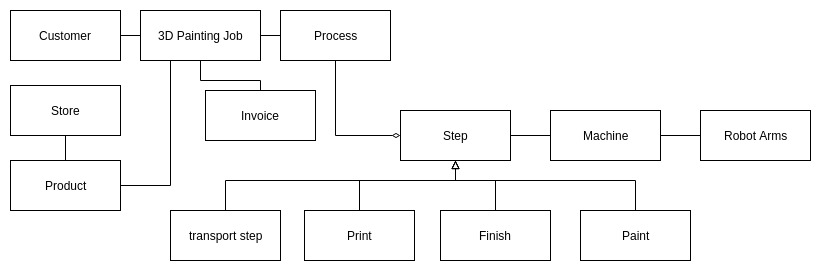
\includegraphics[width=1\textwidth]{01_domain-model}
\caption{Domain-Model}
\end{figure}
\end{frame}

\begin{frame}
\begin{figure}[ht]
\centering
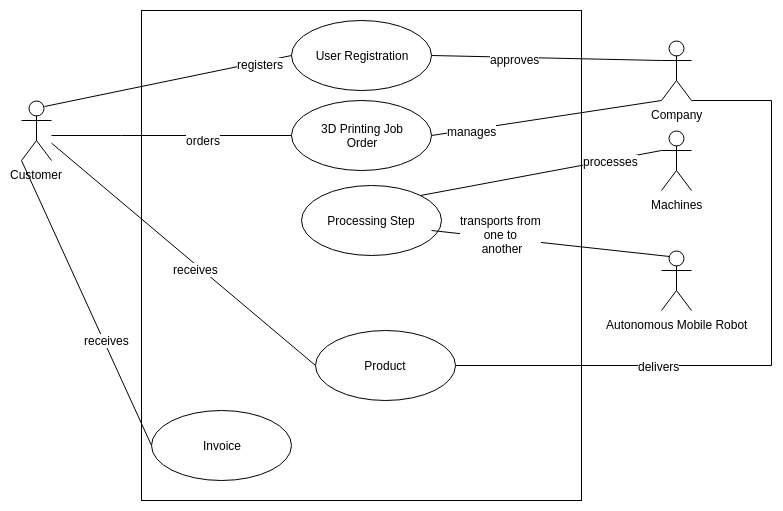
\includegraphics[width=.9\textwidth]{02_use-case}
\caption{Use-Case Diagram}
\end{figure}
\end{frame}

\begin{frame}
\begin{figure}[ht]
\centering
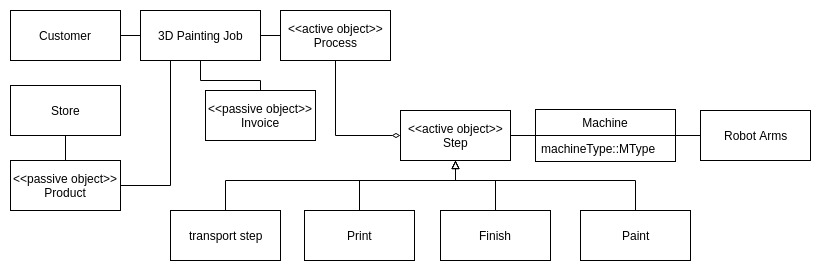
\includegraphics[width=1\textwidth]{03_business-type-model}
\caption{Business Type Model}
\end{figure}
\end{frame}

\begin{frame}
\begin{figure}[ht]
\centering
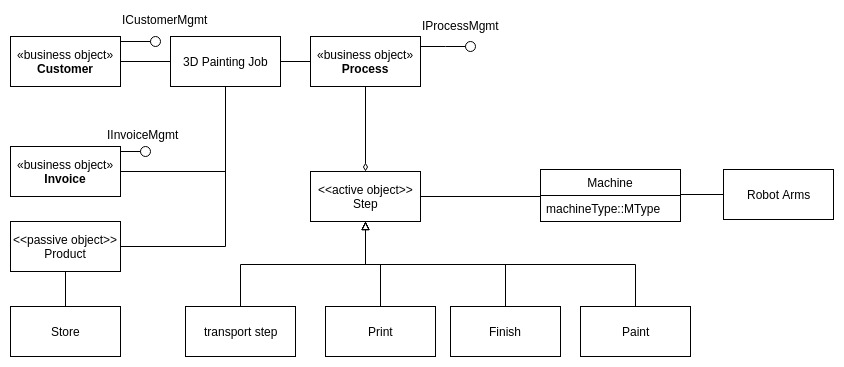
\includegraphics[width=1\textwidth]{04_business-object-interface-model}
\caption{Business Object Interface Model}
\end{figure}
\end{frame}

\begin{frame}
\begin{figure}[ht]
\centering
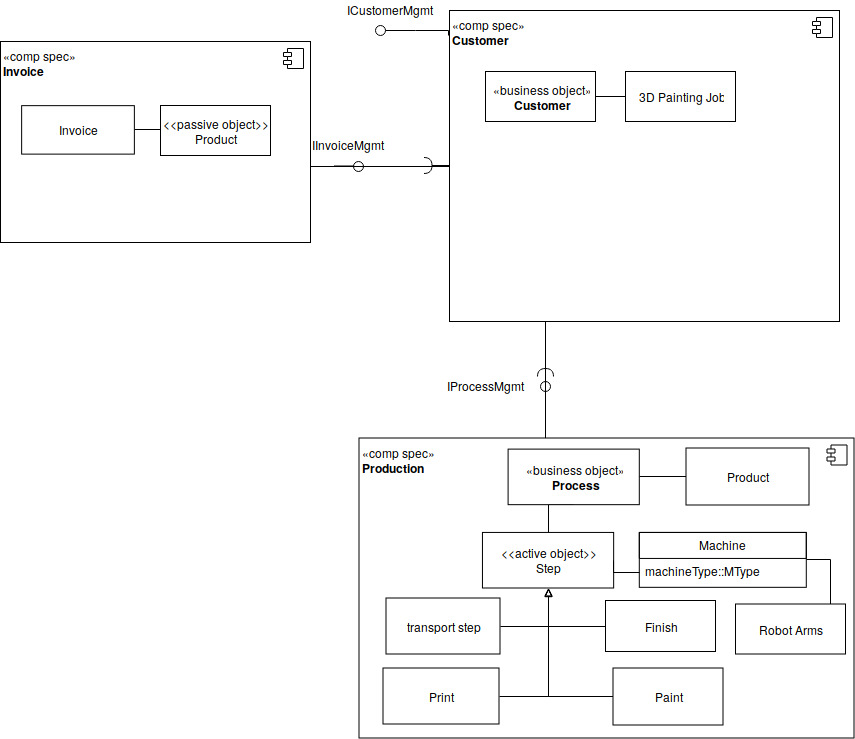
\includegraphics[width=.65\textwidth]{05_component-grouping}
\caption{Component Grouping}
\end{figure}
\end{frame}
\end{document}